\section{Influence of non-uniform variance of features}
\label{section:variances-experiment}

The third experiment is focused on analyzing the impact of the non-standardized features on the performance of the out-of-distribution detection techniques. The research considers such factors as the number of features with modified variance (other than default value: $1.0$) and the modified variance's value itself. Similarly to previous experiment, the number of training samples and dimension of feature vectors are fixed.

\vspace{2.0em}  % NOTE: Just to expand the elements on page a little


\subsection{Experiment organization}
\label{section:variances-organization}

The experiment was organized similarly as the one described in the section \ref{section:distributions-organization}.

The difference lies in the definitions of datasets $T$, $K$ and $U$ – utilizing only one generator $G$ – the Multivariate Normal distribution (MVN). The number of training samples was fixed to $n = 2000$, as well as the dimension of feature vectors $d = 1000$. Instead, there are two new parameters introduced:
\vspace{-0.5\baselineskip}
\begin{itemize}
    \item the fraction of features that have modified (non-default) variance $f_{var}$,
    \item the value of the modified variance $g_{var}$.
\end{itemize}

Both mentioned values affect the content of the covariance matrix $\Sigma$ that is supplied to the MVN generator, e.g., for $d = 6$, $f_{var} = 0.5$ and $g_{var} = 0.25$ it would become
\begin{equation}
    \Sigma_{ID}
    =
    \begin{bmatrix}
        \mathbf{0.25} & 0.00 & 0.00 & 0.00 & 0.00 & 0.00 \\
        0.00 & \mathbf{0.25} & 0.00 & 0.00 & 0.00 & 0.00 \\
        0.00 & 0.00 & \mathbf{0.25} & 0.00 & 0.00 & 0.00 \\
        0.00 & 0.00 & 0.00 & \mathbf{1.00} & 0.00 & 0.00 \\
        0.00 & 0.00 & 0.00 & 0.00 & \mathbf{1.00} & 0.00 \\
        0.00 & 0.00 & 0.00 & 0.00 & 0.00 & \mathbf{1.00}
    \end{bmatrix}
    .
    \label{eq:var-example}
\end{equation}

The features are not correlated here and the default variance of features equals $1.0$.

Only the in-distribution (ID) data (sets $T$ and $K$) are affected by the new parameters. The out-of-distribution (OOD) examples (set $U$) utilizes the identity matrix during generation (i.e., $\Sigma_{OOD} = \mathbb{I}$, features uncorrelated, variance equal to $1.0$).

Summarizing, the input parameters that vary in the experiment are: the fraction of features with non-default variance $f_{var}$, the value of the non-default variance $g_{var}$, the~distance to the outliers $h$ and outlierness measure $OF$. The experiment was repeated several times with various values of the generator seed $\xi$.


\subsection{Experiment results}
\label{section:variances-results}

Third experiment verifies how the outlierness measures perform when affected by the non-uniform variances of features in the dataset, i.e., part of the features in the in-distribution samples utilize a different variance.

Figure \ref{fig:variance} illustrates how the variance value $g_{var}$ influences the performance of outlierness measures. The custom variance value $g_{var}$ is set on a fixed 20\% of features ($f_{var} = 0.2$), while the remaining 80\% features keep the default unitary variance ($1.0$). The experiment involves $n = 2000$ training samples of dimension $d = 1000$ and distance to outliers $h = 16$.

Cases where variance $g_{var} < 1.0$ correspond to concentrated distributions and therefore better spatial separation of data – perfect AUROC score (value $1.0$) is obtained even for IRWD measure (left part of figure \ref{fig:variance-auroc}), leading also to a higher classification accuracy (left part of figure \ref{fig:variance-accuracy}).

The results indicate significant decrease of separability where the custom variance $g_{var} > 1.0$ is applied (right part of figure \ref{fig:variance-auroc}) – especially in case of measures that assume the same significance and values range of each feature: ED, IRWD, kNN and LOF. This situation corresponds to the values of selected 20\% features from in-distribution data overlapping with values for the corresponding features from the out-of-distribution data. Relying on those features leads to losing the ability of proper outliers recognition (specificity) due to too wide spatial distribution of training data – the obtained distance scores for known in-distribution data and out-of-distribution samples start to overlap.

The MD and SED measures take into account the features variances and compensate their contribution to the spatial distance calculation, effectively distinguishing the in-distribution and out-of-distribution data based on the remaining 80\% of features that do not overlap. In the conducted study, SED performs slightly better than MD in the separation task (figure \ref{fig:variance-auroc}) and much better in the classification with respect to the training dataset (\ref{fig:variance-accuracy}). The latter is due to the MD's lack of sensitivity, discussed already in the previous sections of this dissertation (mismatch between scores obtained for training $T$ and testing $K$ in-distribution samples).

It shall be noticed, that due to how the AUROC score calculation is performed\footnote{Implementation detail: the \texttt{roc\_curve()} from scikit-learn library \cite{scikit-learn} assumes higher scores to be associated with a positive label, i.e., treating the scores like the class probability value returned by the classifier; if the scores have different interpretation, like in the conducted study (distance -~lower scores indicate positive class), the function parameters have to be adjusted, e.g., by inverting the labels; \url{https://scikit-learn.org/stable/modules/generated/sklearn.metrics.roc_curve.html}}, for variance value $g_{var} > 2.25$ (figure \ref{fig:variance-auroc}) the unusual value of $\text{AUROC} < 0.5$ can be observed in case of ED, IRWD, kNN and LOF. This corresponds to the distributions histograms visible in the figures \ref{fig:hists-variances-ed}, \ref{fig:hists-variances-knn} and \ref{fig:hists-variances-extreme} – the outlierness scores of in-distribution data are greater (located to the right) than the scores obtained for out-of-distribution data. The interpretation of~that case is: the out-of-distribution data are located closer to the training cluster $T$ center (e.g.~estimated mean) than the actual in-distribution samples. In some of such cases, the fine separability between the in-distribution data and the outliers can be made, such as in figures \ref{fig:hists-variances-extreme-ed} or \ref{fig:hists-variances-extreme-md}. Notably, in cases visible in figures \ref{fig:hists-variances-extreme-ed} and \ref{fig:hists-variances-extreme-sed}, both ED and SED preserve outlierness scores for in-distribution data in the same range, so the very good classification accuracy could be reached if the classification criteria (section \ref{section:verification}, formula \ref{eq:open-set-classification}) would have been revised accordingly.

In some of the observed conditions (figures \ref{fig:hists-variances-knn} and \ref{fig:hists-variances-extreme-md}) it is impossible to reliably calibrate kNN and MD for classification, because the scores obtained for out-of-distribution data are located between scores observed for training and testing in-distribution data.

Figure \ref{fig:n_varied} shows the performance of outlierness measures when a fraction of features $f_{var}$ contains a custom, fixed variance. The fixed variance value is $g_{var} = 1.5$; the remaining fraction of features maintains the default unitary variance ($1.0$). Like in previous example, the results are shown for case involving $n = 2000$ training samples of dimension $d = 1000$ and distance to outliers $h = 16$. The results in this case are analogous the previously discussed case, however now the parameter effect bears stronger impact on all the analyzed measures. Still, both MD and SED perform better than other measures in terms of data separation potential (figure \ref{fig:n_varied-auroc}), as long as the fraction of features with custom variance does not bring the outliers too close to the training data. For $f_{var} = 0.6$ the in-distribution data are non-distinguishable from the outliers for MD and SED; for ED, kNN and LOF the same effect was observed for~$f_{var} = 0.5$.

Overall, the experiment suggests that the analysis of variances and the standardization of data may be necessary to maintain optimal performance of methods such as IRWD, kNN and LOF, while measures like MD or SED work out of the box in the considered scenarios.

\begin{figure}[t]
    \centering
    \begin{subfigure}[b]{0.9\textwidth}
        % StreamLit settings: width=9, height=4
        % X: [0.2, 4.05]
        % Y: [-0.02, 1.02]
        \centering
        \caption{\small Separability between in-distribution and out-of-distribution data}
        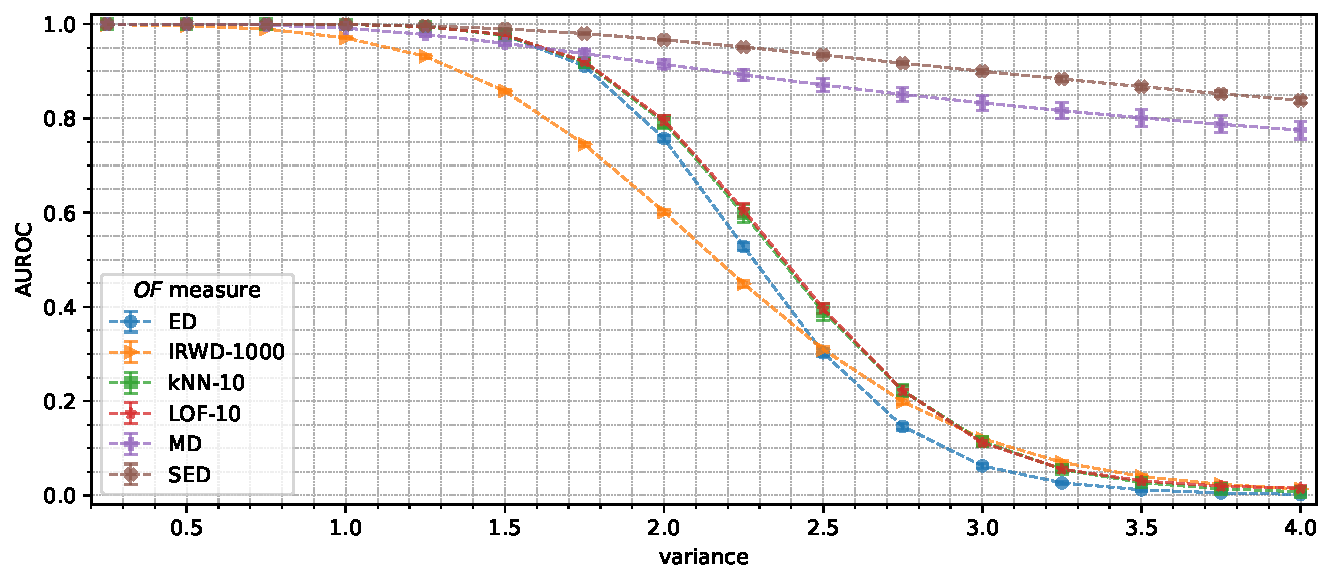
\includegraphics[width=\textwidth]{images/variances/g_var/trend-variances-auroc(variance)-n_varied_0.20-distance_16-outliers_varied_False-model_ED,IRWD-1000,kNN-10,LOF-10,MD,SED-aggregated.pdf}
        \label{fig:variance-auroc}
    \end{subfigure}
    \begin{subfigure}[b]{0.9\textwidth}
        % StreamLit settings: width=9, height=4
        % X: [0.2, 4.05]
        % Y: [0.44, 1.00]
        \centering
        \caption{\small Classification with respect to the training data}
        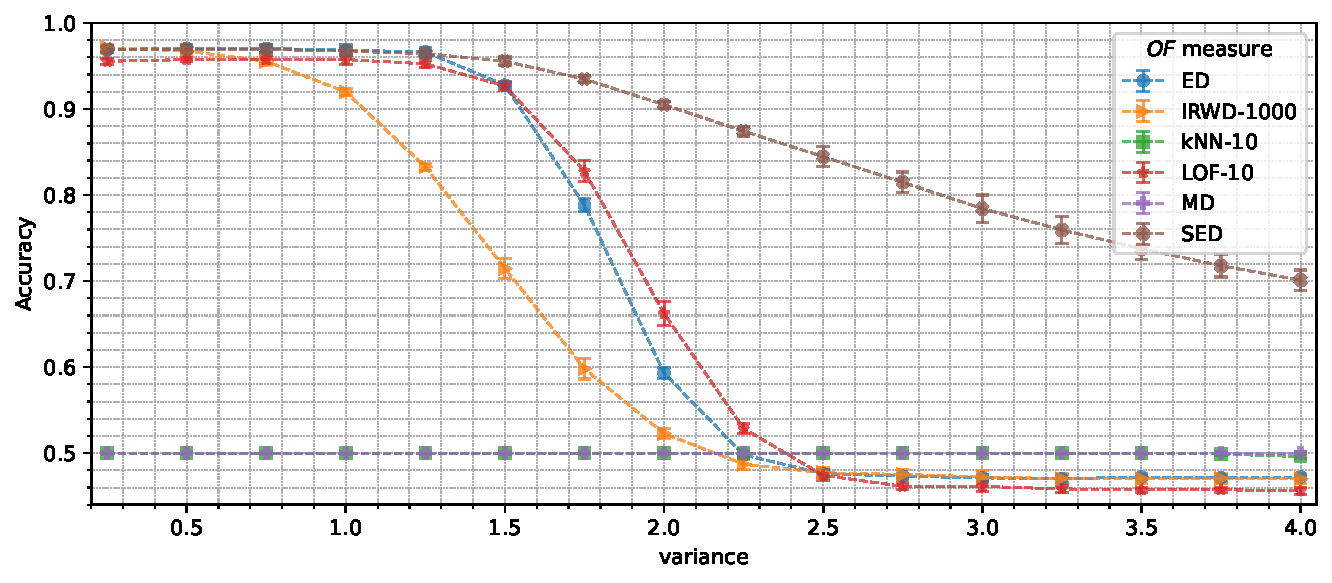
\includegraphics[width=\textwidth]{images/variances/g_var/trend-variances-accuracy_95(variance)-n_varied_0.20-distance_16-outliers_varied_False-model_ED,IRWD-1000,kNN-10,LOF-10,MD,SED-aggregated.pdf}
        \label{fig:variance-accuracy}
    \end{subfigure}
    \begin{subfigure}[b]{0.495\textwidth}
        % StreamLit settings: width=5, height=3
        % X: [0.2, 4.05]
        % Y: [-0.02, 1.05]
        \centering
        \caption{\small Correctly recognized in-distribution}
        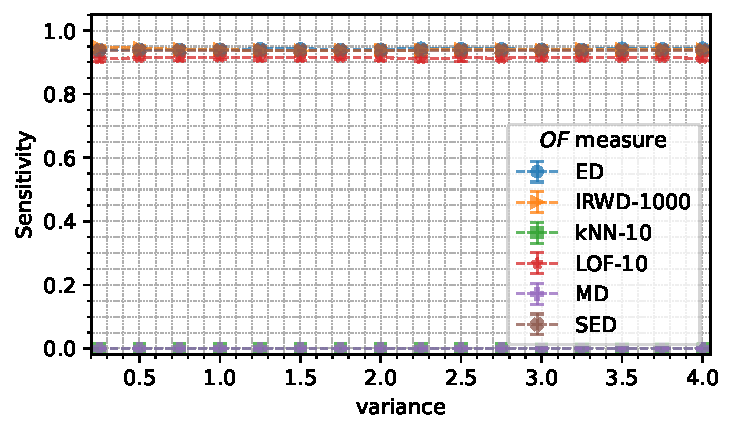
\includegraphics[width=\textwidth]{images/variances/g_var/trend-variances-sens_95(variance)-n_varied_0.20-distance_16-outliers_varied_False-model_ED,IRWD-1000,kNN-10,LOF-10,MD,SED-aggregated.pdf}
        \label{fig:variance-sensitivity}
    \end{subfigure}
    \hfill
    \begin{subfigure}[b]{0.495\textwidth}
        % StreamLit settings: width=5, height=3
        % X: [0.2, 4.05]
        % Y: [-0.02, 1.05]
        \centering
        \caption{\small Correctly recognized out-of-distribution}
        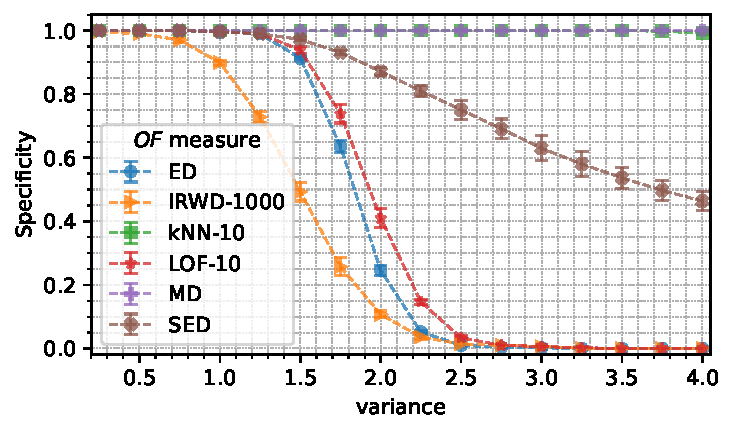
\includegraphics[width=\textwidth]{images/variances/g_var/trend-variances-spec_95(variance)-n_varied_0.20-distance_16-outliers_varied_False-model_ED,IRWD-1000,kNN-10,LOF-10,MD,SED-aggregated.pdf}
        \label{fig:variance-specificity}
    \end{subfigure}
    \caption{The performance of outlierness measures $OF$ as affected by variance of~features value $g_{var}$. The fixed parameters in the experiment are: dimension of~the~feature space $d = 1000$, number of training samples $n = 2000$, distance to~outliers $h = 16$ and fraction of features that have modified variance $f_{var} = 0.2$. The~results~are aggregated for multiple generator seeds $\xi$ and displayed as averages with~error~bars~(standard deviation).}
    \label{fig:variance}
    \vspace{-2.3em}
\end{figure}

\begin{figure}[t]
    \centering
    \begin{subfigure}[b]{0.9\textwidth}
        % StreamLit settings: width=9, height=4
        % X: [-0.01, 1.01]
        % Y: [-0.02, 1.02]
        \centering
        \caption{\small Separability between in-distribution and out-of-distribution data}
        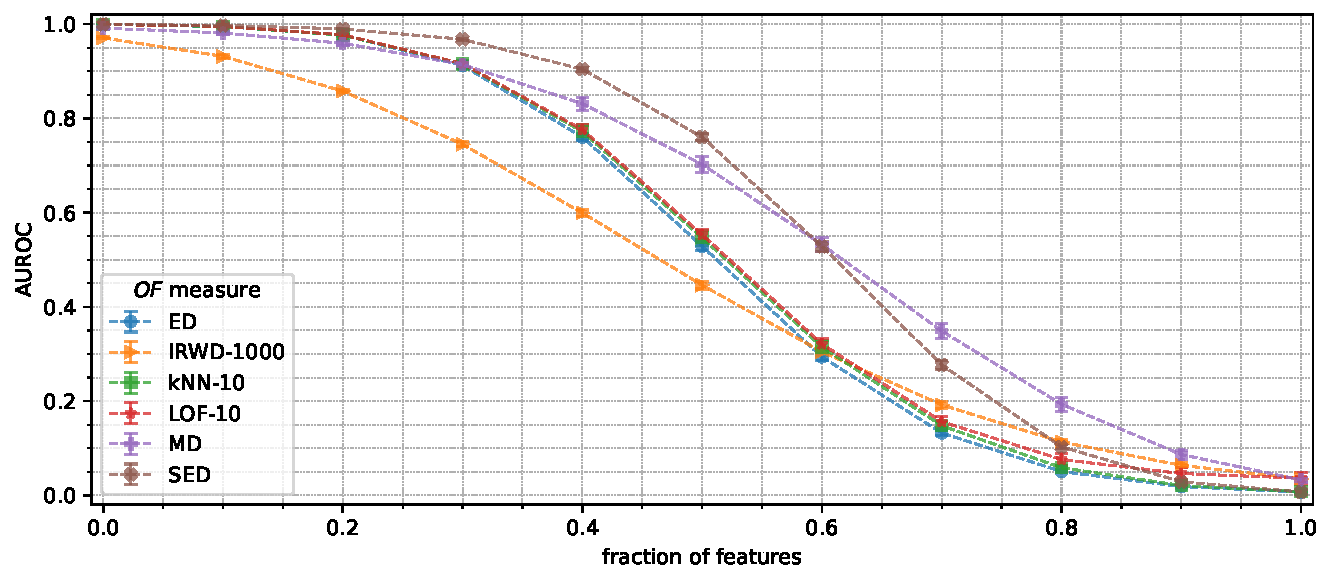
\includegraphics[width=\textwidth]{images/variances/f_var/trend-variances-auroc(n_varied)-variance_1.50-distance_16-outliers_varied_False-model_ED,IRWD-1000,kNN-10,LOF-10,MD,SED-aggregated.pdf}
        \label{fig:n_varied-auroc}
    \end{subfigure}
    \begin{subfigure}[b]{0.9\textwidth}
        % StreamLit settings: width=9, height=4
        % X: [-0.01, 1.01]
        % Y: [0.44, 1.05]
        \centering
        \caption{\small Classification with respect to the training data}
        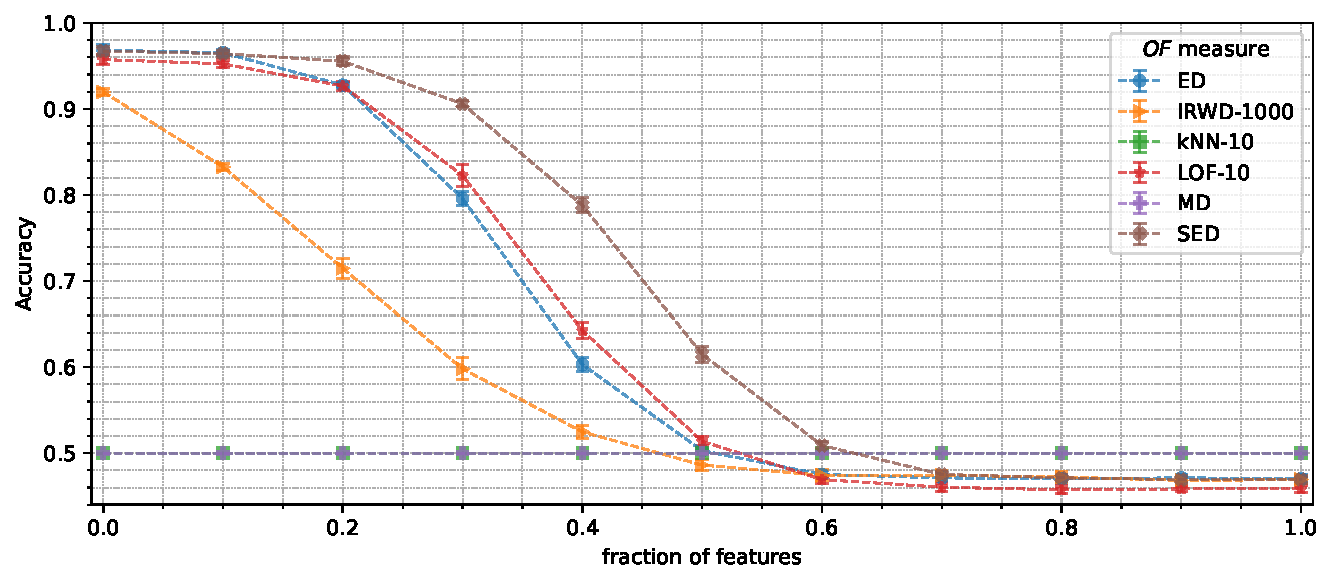
\includegraphics[width=\textwidth]{images/variances/f_var/trend-variances-accuracy_95(n_varied)-variance_1.50-distance_16-outliers_varied_False-model_ED,IRWD-1000,kNN-10,LOF-10,MD,SED-aggregated.pdf}
        \label{fig:n_varied-accuracy}
    \end{subfigure}
    \begin{subfigure}[b]{0.495\textwidth}
        % StreamLit settings: width=5, height=3
        % X: [-0.01, 1.01]
        % Y: [-0.02, 1.00]
        \centering
        \caption{\small Correctly recognized in-distribution}
        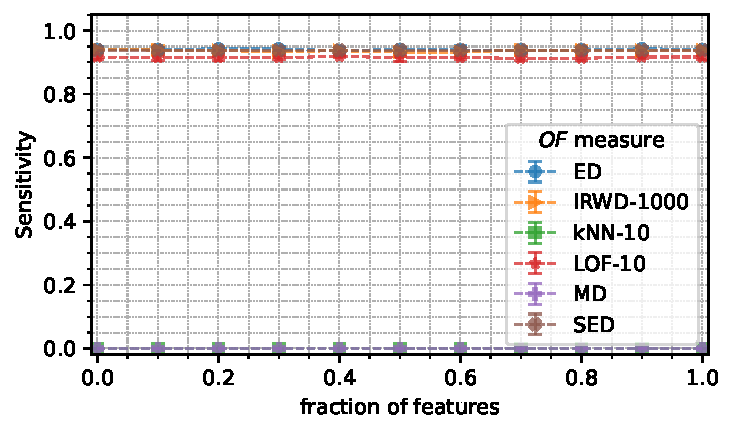
\includegraphics[width=\textwidth]{images/variances/f_var/trend-variances-sens_95(n_varied)-variance_1.50-distance_16-outliers_varied_False-model_ED,IRWD-1000,kNN-10,LOF-10,MD,SED-aggregated.pdf}
        \label{fig:n_varied-sensitivity}
    \end{subfigure}
    \hfill
    \begin{subfigure}[b]{0.495\textwidth}
        % StreamLit settings: width=5, height=3
        % X: [-0.01, 1.01]
        % Y: [-0.02, 1.05]
        \centering
        \caption{\small Correctly recognized out-of-distribution}
        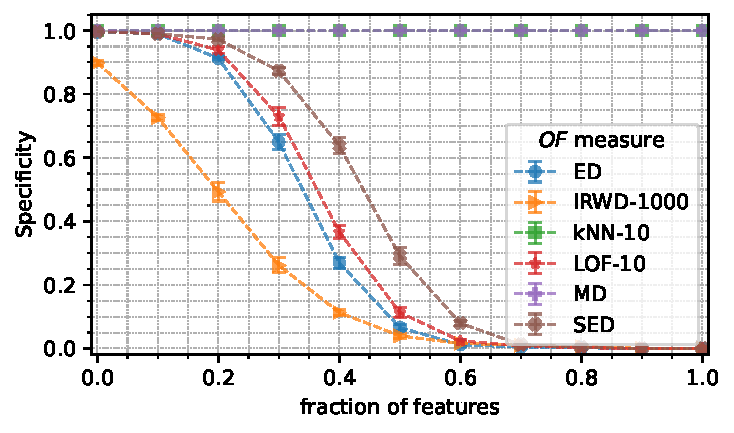
\includegraphics[width=\textwidth]{images/variances/f_var/trend-variances-spec_95(n_varied)-variance_1.50-distance_16-outliers_varied_False-model_ED,IRWD-1000,kNN-10,LOF-10,MD,SED-aggregated.pdf}
        \label{fig:n_varied-specificity}
    \end{subfigure}
    \caption{The performance of outlierness measures $OF$ as affected by the fraction of features that have modified variance $f_{var}$. The fixed parameters in the experiment are: dimension of the feature space $d = 1000$, number of training samples $n = 2000$, distance to outliers $h = 16$ and variance of~features value $g_{var} = 1.5$. The~results are aggregated for multiple generator seeds $\xi$ and displayed as averages with~error~bars~(standard deviation).}
    \label{fig:n_varied}
    \vspace{-2.3em}
\end{figure}

\begin{figure}[t]
    % StreamLit settings: width=9, height=2
    \centering
    \begin{subfigure}[b]{\textwidth}
        \centering
        \caption{\small Euclidean distance, variance: $g_{var} = 3.0$, fraction: $f_{var} = 0.2$}
        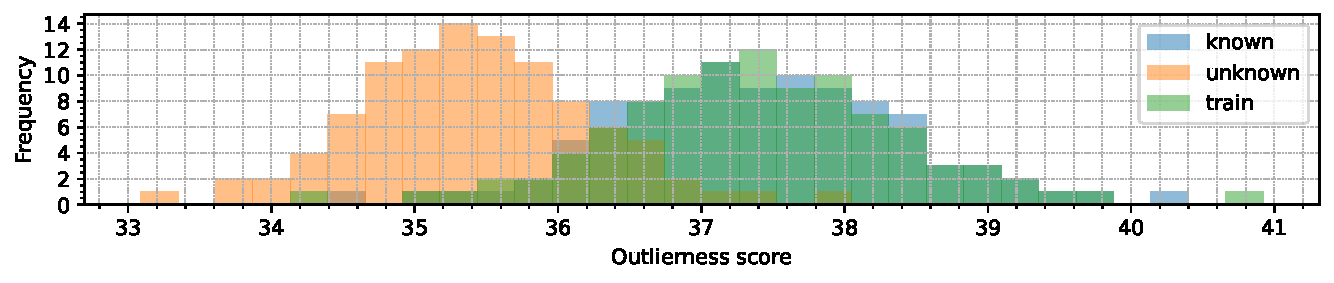
\includegraphics[width=\textwidth]{images/variances/hists/hist-variances-n_varied_0.20-variance_3.00-distance_16-outliers_varied_False-model_ED-seed_0.pdf}
        \label{fig:hists-variances-ed}
    \end{subfigure}
    \begin{subfigure}[b]{\textwidth}
        \centering
        \caption{\small k-Nearest Neighbors ($k=10$), variance: $g_{var} = 3.0$, fraction: $f_{var} = 0.2$}
        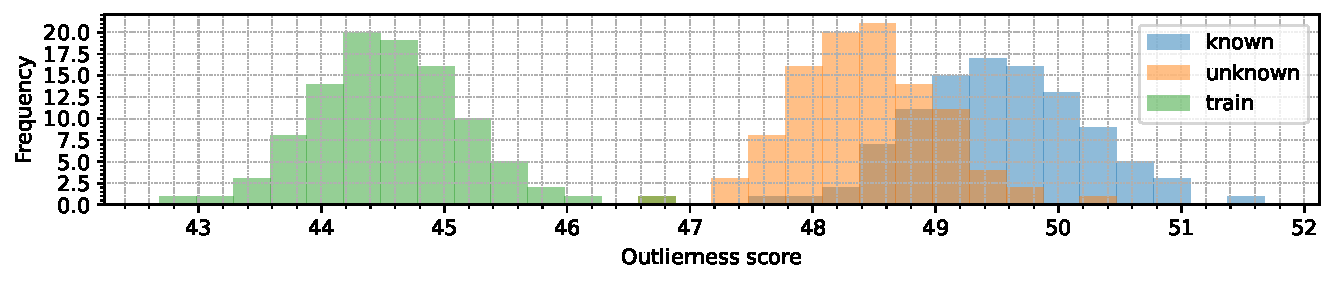
\includegraphics[width=\textwidth]{images/variances/hists/hist-variances-n_varied_0.20-variance_3.00-distance_16-outliers_varied_False-model_kNN-10-seed_0.pdf}
        \label{fig:hists-variances-knn}
    \end{subfigure}
    \begin{subfigure}[b]{\textwidth}
        \centering
        \caption{\small Mahalanobis distance, variance: $g_{var} = 3.0$, fraction: $f_{var} = 0.2$}
        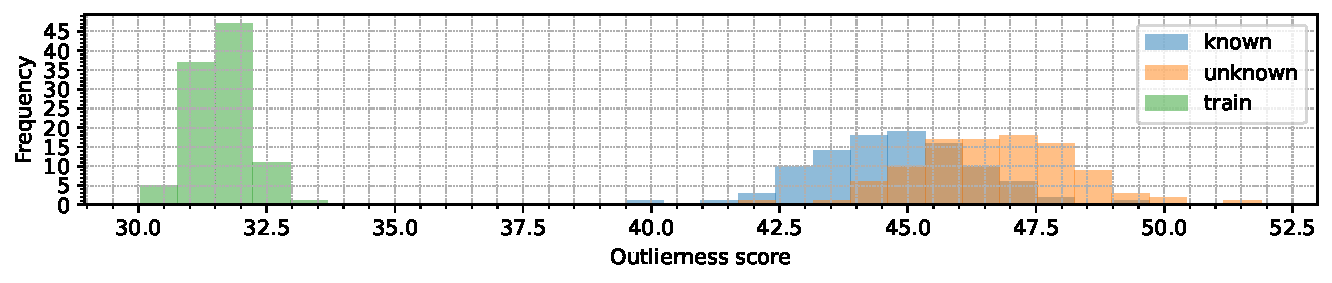
\includegraphics[width=\textwidth]{images/variances/hists/hist-variances-n_varied_0.20-variance_3.00-distance_16-outliers_varied_False-model_MD-seed_0.pdf}
        \label{fig:hists-variances-md}
    \end{subfigure}
    \begin{subfigure}[b]{\textwidth}
        \centering
        \caption{\small Standardized Euclidean distance, variance: $g_{var} = 3.0$, fraction: $f_{var} = 0.2$}
        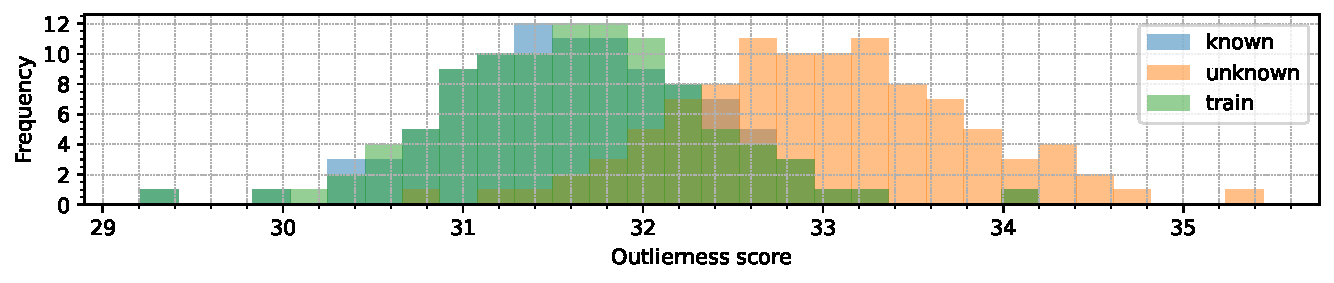
\includegraphics[width=\textwidth]{images/variances/hists/hist-variances-n_varied_0.20-variance_3.00-distance_16-outliers_varied_False-model_SED-seed_0.pdf}
        \label{fig:hists-variances-sed}
    \end{subfigure}
    \caption{Histograms of outlierness scores for various measures $OF$ considering data distribution with a~small fraction of features having bigger variance. Due to bigger variance the outliers starts to overlap with in-distribution data in space, yet measures that consider the variance (MD, SED) maintain the ability to separate the clusters, while for kNN the outliers appear closer to training data than the known in-distribution examples. Other experiment parameters involved: dimension of feature space $d = 1000$, number of~training samples $n = 2000$, distance~to~outliers $h = 16$, generator seed $\xi = 0$.}
    \label{fig:hists-variances}
\end{figure}

\begin{figure}[t]
    % StreamLit settings: width=9, height=2
    \centering
    \begin{subfigure}[b]{\textwidth}
        \centering
        \caption{\small Euclidean distance, variance: $g_{var} = 4.0$, fraction: $f_{var} = 0.5$}
        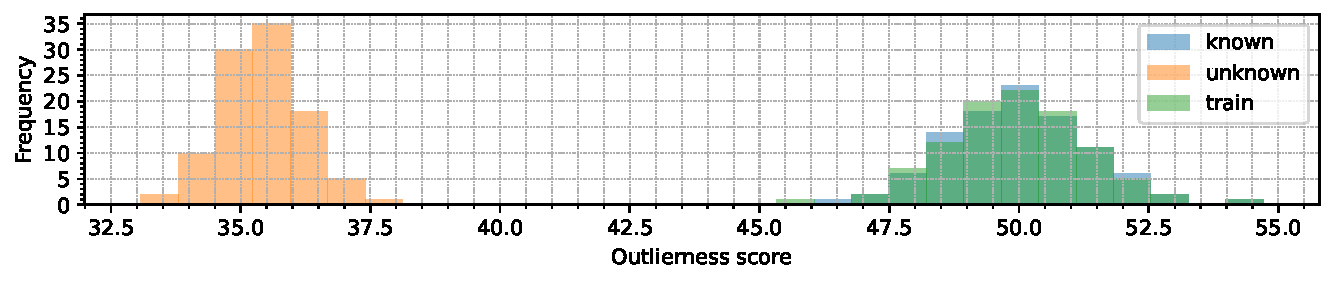
\includegraphics[width=\textwidth]{images/variances/hists-extreme/hist-variances-n_varied_0.50-variance_4.00-distance_16-outliers_varied_False-model_ED-seed_0.pdf}
        \label{fig:hists-variances-extreme-ed}
    \end{subfigure}
    \begin{subfigure}[b]{\textwidth}
        \centering
        \caption{\small k-Nearest Neighbors ($k=10$), variance: $g_{var} = 4.0$, fraction: $f_{var} = 0.5$}
        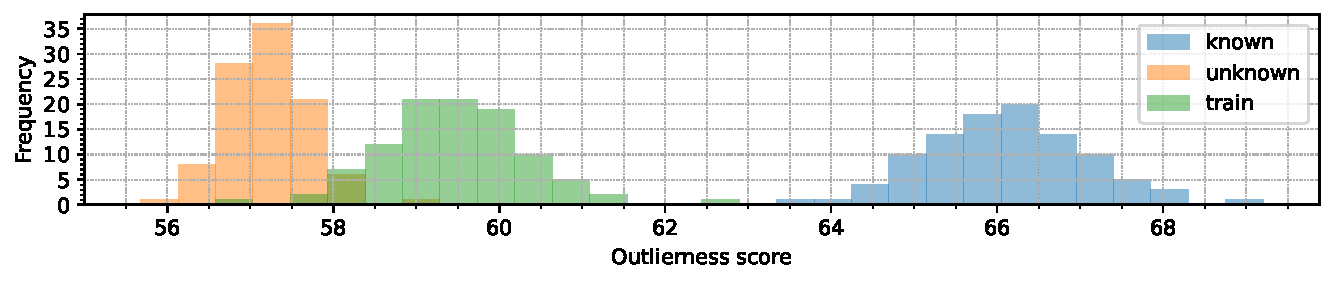
\includegraphics[width=\textwidth]{images/variances/hists-extreme/hist-variances-n_varied_0.50-variance_4.00-distance_16-outliers_varied_False-model_kNN-10-seed_0.pdf}
        \label{fig:hists-variances-extreme-knn}
    \end{subfigure}
    \begin{subfigure}[b]{\textwidth}
        \centering
        \caption{\small Mahalanobis distance, variance: $g_{var} = 4.0$, fraction: $f_{var} = 0.5$}
        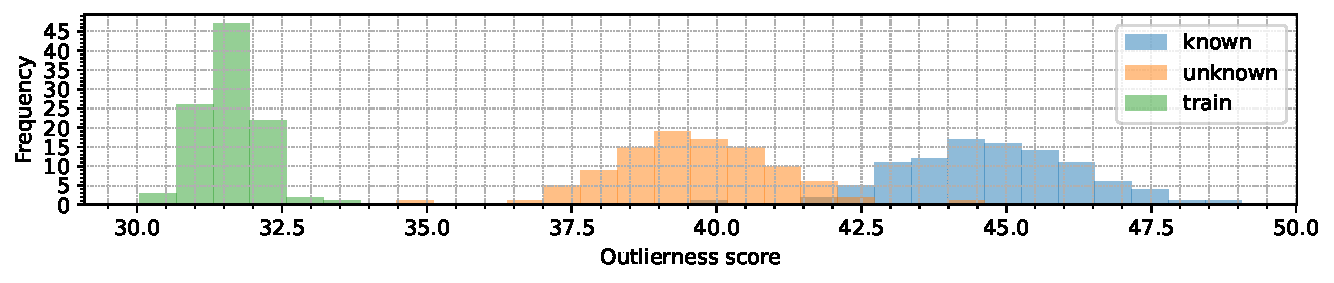
\includegraphics[width=\textwidth]{images/variances/hists-extreme/hist-variances-n_varied_0.50-variance_4.00-distance_16-outliers_varied_False-model_MD-seed_0.pdf}
        \label{fig:hists-variances-extreme-md}
    \end{subfigure}
    \begin{subfigure}[b]{\textwidth}
        \centering
        \caption{\small Standardized Euclidean distance, variance: $g_{var} = 4.0$, fraction: $f_{var} = 0.5$}
        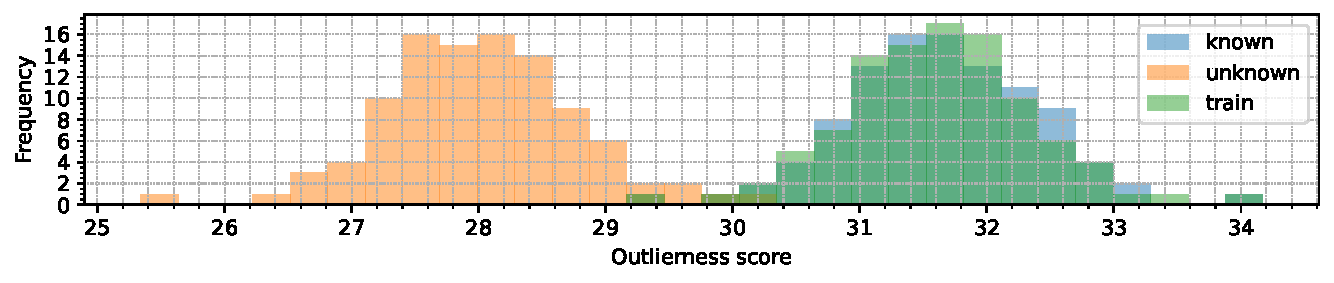
\includegraphics[width=\textwidth]{images/variances/hists-extreme/hist-variances-n_varied_0.50-variance_4.00-distance_16-outliers_varied_False-model_SED-seed_0.pdf}
        \label{fig:hists-variances-extreme-sed}
    \end{subfigure}
    \caption{Histograms of outlierness scores for various measures $OF$ considering data distribution with a~significant fraction of features having very big variance. In~such conditions it is impossible to reliably calibrate kNN and MD for classification, while both ED and SED preserve scores for in-distribution data in the same range (however, the formula \ref{eq:open-set-classification} would have to be revised for classification). Other experiment parameters involved: dimension of feature space $d = 1000$, number of~training samples $n = 2000$, distance~to~outliers $h = 16$, generator seed $\xi = 0$.}
    \label{fig:hists-variances-extreme}
\end{figure}

\cleardoublepage{}
